\clearpage
\section{Segunda parte del Módulo de usuarios}
    \begin{description}
        \item \textbf{Duración}: 15 días.
        \item \textbf{Inicio del sprint }: .
        \item \textbf{Cierre del sprint }: .
    \end{description}

Esta iteración tuvo como propósito terminar de implementar todo el el modulo completo de usuarios:
\begin{enumerate}
    \item Se 
\end{enumerate} 

Los requerimientos funcionales de este sprint se muestran en la siguiente tabla.
\begin{requerimientos}{funcionales}
    \RFitem{}{}{}
\end{requerimientos}

Los casos de uso que se describieron en este sprint pertenecen al \textbf{Módulo } 

En la figura \ref{dcu:DCUPST} se puede ver el diagrama de casos de uso.
\begin{itemize}
    \item Los casos de uso \IUazul{} , son aquellos que se van implementar en este sprint.
    \item Los casos de uso \IUblanco{}, se tienen planeados para sprints posteriores.
\end{itemize} 

\begin{figure}[H]
    \begin{center}
        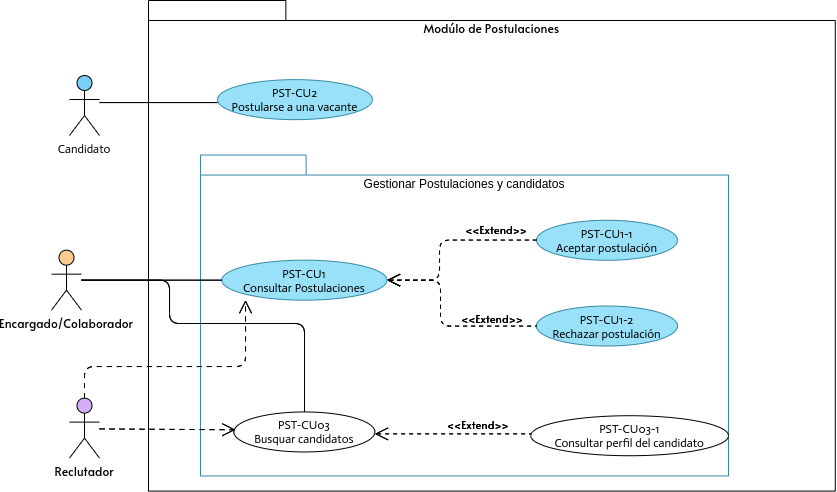
\includegraphics[width=.7\textwidth]{sprints/imagenes/DCUPST.png}
    \end{center}
    \caption{Diagrama de casos de uso del \textit{Modúlo Postulaciones}.}
    \label{dcu:DCUPST}
\end{figure}

Los casos de uso que se implementaron en este sprint fueron:
\begin{enumerate}
    \item \refElem{USR-CU02}
    \item \refElem{PST-CU01-1}
    \item \refElem{PST-CU01-2}
\end{enumerate} 



Para la construcción del módulo de gestión de postulaciones se construyeron servicios para realizar la comunicación entre frontend y backend, y de esta forma hacer la peticiones HTTP con el verbo GET a cada endpoint que almacena la información de una postulación, ya sea las de postulaciones que realiza un candidato a una vacante o la lista postulaciones de candidatos que recibe el reclutador peticiones HTTP con el verbo POST al endpoint que solicita agregar los registros de postulaciones a una vacante y peticiones HTTP con el verbo PUT para actualizar el estado de la postulación y, de ser necesario, actualizar el estado de la vacante.\\
\newline
Cuando se realiza una postulación se revisa antes el usuario que intenta aplicar a la vacante no tenga otra postulación en proceso a la misma vacante, es decir, se verifica que no se haya postulado anteriormente o si se ha postulado ese intento ya haya sido descartado. Cuando se corroboró que la postulación es válida, se genera un registro enlazado al usuario y a la vacante a la que aplicó para tener control del estado de su postulación, así mismo se genera un estado inicial de la vacante para controlar los cambios que ha tenido la solicitud. Al cambiar el estado de cualquier postulación se verifica que el estado de la  vacante a la que hace referencia la postulación no cambie a causa del cambio en la postulación, de ser así, entonces se actualiza el estado de la vacante para que coincida con el estado al que corresponda y así tener siempre actualizada la información mostrada a los usuarios.
